% !TEX root = ../../CompVis.tex
\section{Network Architectures}
\begin{minipage}{0.5\textwidth}
    \subsection{LeNet (from 1998)}
    Used for handwritten digit recognition. Uses 2 convolutional layers 2 pooling (averaging) layers.

    \subsection{AlexNet (2012)}
    5 Convolutional layers, max-pooling, 3 fully connectec layers, ReLU activation $\rightarrow$ 60 million parameters (!)
\end{minipage}
\begin{minipage}{0.5\textwidth}
    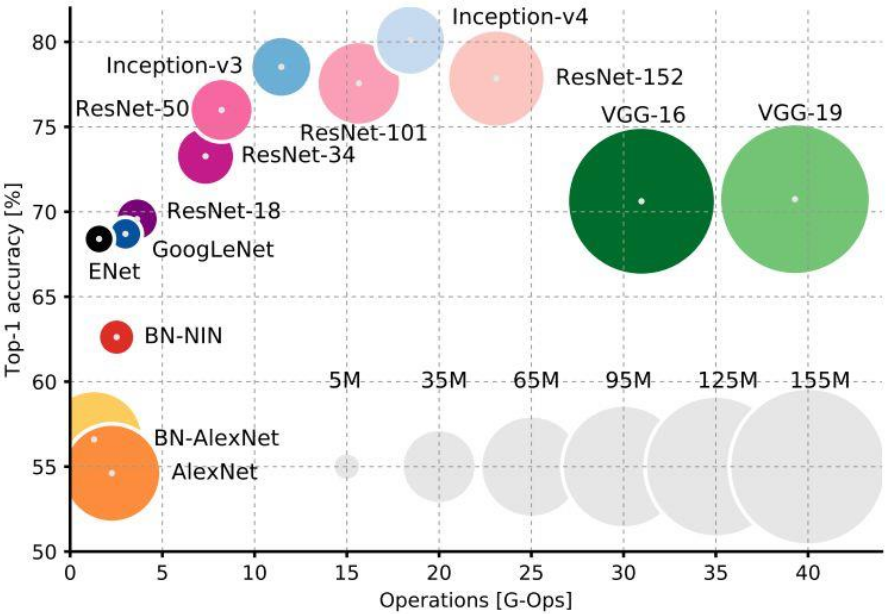
\includegraphics[width=\textwidth]{sections/NetworkArchitectures/img/accuracy_on_imagenet.png}
\end{minipage}


\subsection{GoogLeNet}
\begin{minipage}{0.5\textwidth}
    New architecture with filters of various sizes (inception network)
    \begin{itemize}
        \item 22 layers deep (layers with parameters)
        \item ca. 100 layer building blocks
    \end{itemize}
\end{minipage}
\begin{minipage}{0.5\textwidth}
    \centering
    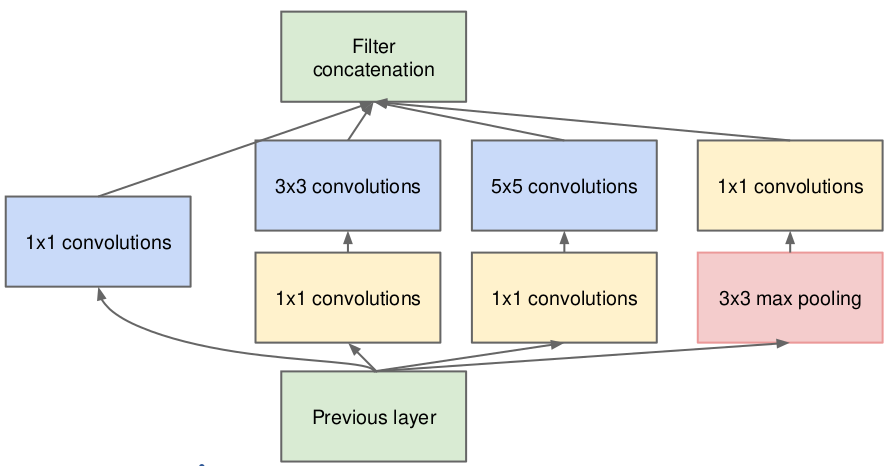
\includegraphics[width=0.8\textwidth]{sections/NetworkArchitectures/img/googlenet_various_sizes}
\end{minipage}

\subsection{VGG Net}
Only $3\times 3$ convolutional layers, some with pooling. $\rightarrow$ Stack of $3\times 3$ filters has the same receptive field as a $7\times 7$ filter, but less parameters and more non-linearity

\subsection{ResNet}
\begin{minipage}{0.7\textwidth}
    \begin{itemize}
        \item Networs get deeper: If there are enough layers, adding more should not decrease performance.
        \item Layers do not learn identity transform easily $\rightarrow$ use residual connections
        \item For deeper networks also use bottlenck layer to improve efficiency
    \end{itemize}
\end{minipage}
\begin{minipage}{0.3\textwidth}
    \centering
    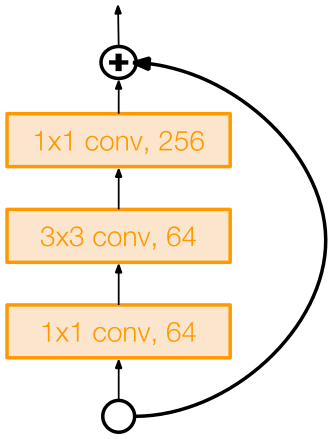
\includegraphics[width=0.6\textwidth]{sections/NetworkArchitectures/img/resnet}
\end{minipage}


\subsubsection{Inception ResNet v2}
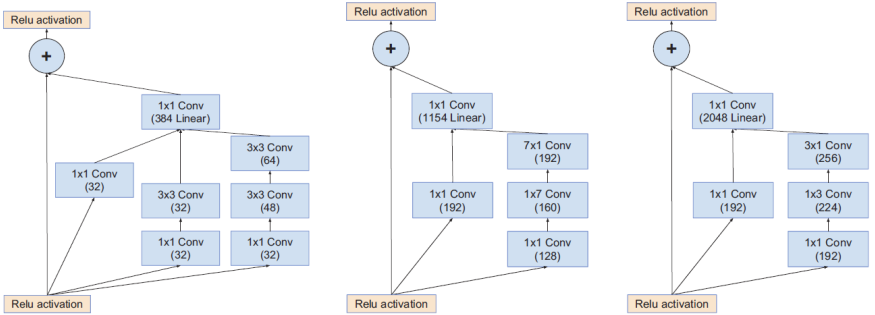
\includegraphics[width=\textwidth]{sections/NetworkArchitectures/img/inception_resnet.png}
